\documentclass{article}

\usepackage{amssymb,amstext,amsmath,graphicx,float,subfig,array,hyperref}
\usepackage[hmargin=3cm,vmargin=3.5cm]{geometry}

\begin{document}

\title{Lunar Impact: A Modest Proposal}
\author{Ricardo Medina}
\date{\today \\ 
\bigskip
This report has been prepared in accordance with the honor code of
Brown University.
The report and MATLAB code are my own work}

\maketitle
\thispagestyle{empty}
\pagebreak

\tableofcontents

\pagebreak

\begin{abstract}
  Using the European Space Agency's Ariane V as a launch system,
  satellites may be jettisoned into a geosynchronous transfer orbit
  that matches the parameter's of Ariane V's own orbit.
  This paper documents how available
  information about the moon and Ariane V may be used to design a
  mission that could take a satellite and have it impact the moon
  given only a single finite and contiguous increase in speed (acting
  in the direction of the satellite's motion).
  
  I describe in detail the methods, data, and calculations used
  to determine when the satellite should be launched and what that
  change in its speed should be.

  The goal is to prove, that a launch on 13 April, 2011, with a speed
  increase of 0.703 km/s would yield a successful impact to the moon
  from a Ariene V's GTO with an impact velocity of 2.682 km/s.
\end{abstract}

\section{Introduction}
Indeed, impacting the Earth's moon, which is between 356,575.001 km and
406,656.171 km away from the Earth, is no trivial task. The process of
finding design parameters that would yield a successful mission
involved a bit of guessing as well as several refining processes to
increase the general accuracy of the results.

Even the most basic task, that of deciding on governing equations of
motion was a somewhat iterative process.
Initially, the effect of the moon's gravity on the satellite was
ignored. Nevertheless, this produces a useful sense of how long it
will take the satellite to travel to the moon given the change in
velocity. Once I implemented more precise conditions and equations
(the processes for which are described in subsequent sections),
the proper trajectory and impact velocity can be determined.

\section{Mission Calculations}
\subsection{Equations of Motion}\label{sec:motion}

The force due to the Earth's gravity on a body in space is:
\begin{equation}
  \vec{F} = -\frac{GM_em}{r^2}\frac{\vec{r}}{r} =
  -\frac{GM_em}{r^3}\langle x, \; y, \; z \rangle = m\vec{a},
\end{equation}
where $m$ is the mass of the body orbiting the earth, $M_e$ is the
mass of the earth, $r$ is the distance from the center of the earth to
the body, and $\vec{r} = \langle x, \; y, \; z \rangle$ is the position vector
of the body with $i, j,$ and $k$ components. Thus:
\begin{align}
  -\frac{GM_em}{r^3}\langle x \; y \; z \rangle &= m\langle \frac{d^2x}{dt}, \;
  \frac{d^2y}{dt}, \;  \frac{d^2z}{dt} \rangle \intertext{and} \\
  \therefore \; -\frac{GM_e}{r^3}\langle x \; y \; z \rangle &= \langle \frac{d^2x}{dt}, \;
  \frac{d^2y}{dt}, \;  \frac{d^2z}{dt} \rangle. \label{eq:eomsimp}
\end{align}

Clearly, this does not show the whole
picture. Equation.(\ref{eq:eomsimp}) ignores any and all other bodies in
space and assumes that the Earth is stationary. These are by no means
unreasonable assumptions for the moon, but do not accurately predict a
trajectory for the satellite which has the moon's gravity pulling on
it as well.

The force due to the moon's gravity on the satellite is:
\begin{equation}
  \vec{F_{ms}} = \frac{GM_mm_s}{r_{sm}^2}\frac{\vec{r_{sm}}}{r_{sm}} =
  \frac{GM_mm}{r_{sm}^3}\langle x_{sm}, \; y_{sm}, \; z_{sm} \rangle,
\end{equation}
Here, $\vec{F_{ms}}$ is the force of the moon on the satellite,
$M_m$ is the moon's mass, $\vec{r_{sm}}$ is the position
vector of the moon minus the position vector of the satellite (the
direction that this vector points in is the reason that the force
expression has no negative sign), $r_{sm}$ is the magnitude of that
vector, and $\langle x_{sm}, \; y_{sm}, \; z_{sm} \rangle,$ are its
$i,j,$ and $k$ components. The total force, then, on the satellite
is:

\begin{align}
  \vec{F_{s}} = -\frac{GM_e}{r^3}\langle x_s \; y_s \; z_s \rangle +
  \frac{GM_mm}{r_{sm}^3}\langle x_{sm}, \; y_{sm}, \; z_{sm} \rangle,
\end{align}

Matlab cannot strictly solve for second order differential
equations. Without the lunar gravitation considerations, the initial
conditions, the initial conditions can be passed to a function that
outputs the following array:
\begin{equation}
  \frac{d}{dt}
  \begin{bmatrix}
    x \\ y \\ z \\ v_x \\ v_y \\ v_z
  \end{bmatrix} =
  \begin{bmatrix}
    v_x \\ v_y \\ v_z \\
    -GM_ex/r^3 \\
    -GM_ey/r^3 \\
    -GM_ez/r^3.
  \end{bmatrix}
\end{equation}
From this, it is clear that initial values for $x, y, z, v_x, v_y,
v_z$ are needed in order to get usable result. For the satellite, we
are assuming that it starts at perigee, and for the sake of plotting
the moon, the same will be assumed. The appropriate code can be found
in Appendix.\ref{sec:eomcode}.

When the code is extended to
include the more accurate force expressions on the satellite, the
appropriate array looks more like:
\begin{equation}
  \frac{d}{dt}
  \begin{bmatrix}
    x_s \\ y_s \\ z_s \\ v_{xs} \\ v_{ys} \\ v_{zs} \\
    x_m \\ y_m \\ z_m \\ v_{xm} \\ v_{ym} \\ v_{zm}
  \end{bmatrix} =
  \begin{bmatrix}
    v_{xs} \\ v_{ys} \\ v_{zs} \\
    -GM_ex_s/r^3+GM_mx_{sm}/r_{sm}^3 \\
    -GM_ey_s/r^3+GM_my_{sm}/r_{sm}^3 \\
    -GM_ez_s/r^3+GM_my_{sm}/r_{sm}^3 \\
    v_{xm} \\ v_{ym} \\ v_{zm} \\
    -GM_ex_m/r^3 \\
    -GM_ey_m/r^3 \\
    -GM_ez_m/r^3.
  \end{bmatrix}
  \label{eq:eom}  
\end{equation}
It is important to note that these need to be solved simultaneously.

\subsection{Lunar Orbit}

In order to crash a satellite into the moon, one of the first obvious
tasks is to know a precise location for the moon as a function of
time.
As a result, available data had to be interpreted and manipulated to
obtain information that would be useful to some second-order
differential equation that governs its motion (Equation.(\ref{eq:eom})).
The information available on the Naval Oceanography Portal's
website \cite{USNO}
comes in the following format:
\\
\noindent
\begin{table}[H]\centering
\begin{tabular}{r r r r r r r r r r r}
  \multicolumn{2}{l}{Date} & Time & \multicolumn{3}{l}{Right Ascension} &
  \multicolumn{4}{l}{Declination} & Distance \\ 
  \hline
  & & h:m:s & h & m & s & & $^\circ$ & $\prime$ & $\prime\prime$ & km
  \\ 
  Mar & 13 & 00:00:00.0 & 5 & 25 & 49.818 & + & 23 & 46 & 15.22 &
  387576.328 \\
  Mar & 13 & 01:00:00.0 & 5 & 28 & 10.483 & + & 23 & 45 & 16.59 &
  387337.528 \\
  Mar & 13 & 02:00:00.0 & 5 & 30 & 31.285 & + & 23 & 44 & 9.93 &
  387097.693 \\
  Mar & 13 & 03:00:00.0 & 5 & 32 & 52.219 & + & 23 & 42 & 55.20 &
  386856.844 \\
  Mar & 13 & 04:00:00.0 & 5 & 35 & 13.283 & + & 23 & 41 & 32.39 &
  386615.001 \\
  Mar & 13 & 05:00:00.0 & 5 & 37 & 34.473 & + & 23 & 40 & 1.47 &
  386372.187 \\
  Mar & 13 & 06:00:00.0 & 5 & 39 & 55.784 & + & 23 & 38 & 22.44 &
  386128.422 \\
  Mar & 13 & 07:00:00.0 & 5 & 42 & 17.214 & + & 23 & 36 & 35.26 &
  385883.729 \\
  Mar & 13 & 08:00:00.0 & 5 & 44 & 38.758 & + & 23 & 34 & 39.93 &
  385638.130 \\
  Mar & 13 & 09:00:00.0 & 5 & 47 & 0.413 & + & 23 & 32 & 36.44 &
  385391.647 \\
\end{tabular}
\caption{This is a sample of data taken from the website where the
  starting date was March 13, 2011, and the interval between data points
  is an hour}
\label{tab:sampledata}  
\end{table}

The entire query made to the website returned 3000 consecutive hours worth
of lunar locations.
The co\"ordinates are given in a pseudo-spherical way where the
compliment of the declination, $\delta$, is the polar angle, the right
ascension, $\alpha$, is the azimuthal angle, and distance is the radial
component. In order, then, to get Cartesian co\"ordinates from this,
one needs to multiply the distance, $r$, by some vector:
\begin{equation}
  \langle \cos{\alpha}\cos{\delta}, \; \sin{\alpha}\cos{\delta}, \;
  \sin{\delta} \rangle.
\end{equation}

It was known that one can solve for the position of the moon as a
function of time by knowing an initial location and velocity (among
other things discussed in Section.\ref{sec:motion}). To find these initial conditions:
\begin{align}
  \vec{r} &= \rho \langle \cos{\alpha}\cos{\delta}, \;
  \sin{\alpha}\cos{\delta}, \; \sin{\delta} \rangle
  \label{eq:rmoon}, \\
  \vec{v_p} &=
  (2\mu\frac{\rho_a}{\rho_p(\rho_a+\rho_p)})^{\frac{1}{2}}
  \frac{\vec{m}\times\vec{r_p}}{\rho_p},
\end{align}
where $\vec{r}$ is the position vector when the moon is at some point,
$\rho$ is the distance of the moon at that point from the center of
the earth plus the radius of the moon,
$\mu$ is a gravitational parameter that
is the product of the gravitational constant and the mass of the
earth, $\vec{v_p}$ is the velocity of the moon at perigee,
$\rho_p$ is the distance of the moon at perigee to the center
of the earth plus the radius of the moon, $\rho_a$ is the distance of the moon to the center of the earth
at apogee plus the radius of the moon, and $\vec{m}$ is some unit vector normal to the plane of the
moon's orbit. The desired $\vec{r}$ is when the moon is at perigee.

In order to do this in MatLab, a function \verb[moondata[, Appendix.\ref{sec:moonorb}, that
outputs $\vec{r_p}, \vec{v_p}, \rho_p$,$\rho_a$ and takes 2 arguments,
a file and the gravitational parameter was made and used.
The file passed to this function
is a \verb[.csv[ that contains the $\alpha,\delta,r$ of all the
data points. Because of limitations in Matlab, the $\pm$ in the
declination need to have a 1 appended to the end of that field. All
data processing was done in bash using \verb[sed[.

So, what the function does is take the file argument and make it an
array whereby it finds the maximum and minimum values for the last
field. It stores these values and takes the other fields in that index
and passes it to another function that then stores the $\alpha$ and
$\delta$ values in radians for when the moon is at perigee and apogee.
From this, $\vec{r_p}$ can be found easily with Equation.(\ref{eq:rmoon}).

To find $\vec{m}$, the cross product of $\vec{r_p}$ and $\vec{r_a}$
divided by their norm produces the correct vector. Hence, the position
and velocity at perigee is known for later use.

\subsection{Satellite Orbit}

As stated in A.2, data about satellite orbit, in particular ARIANE
GTO, comes as 5 pieces of information: inclination, $\theta$, altitude of
periapsis, $r_p$, altitude of apoapsis, $r_a$, longitude of first
ascending node, $\Omega$, and the argument of the periapsis, $\omega$.

According to A.6, these values are: \\
\begin{tabular}{|l|c|}
  \hline
  Inclination & 7 degrees \\ \hline
  Altitude of perigee & 250 km \\ \hline
  Altitude of apogee & 35950 km\\ \hline
  Argument of perigee & 178 degrees \\ \hline
  Longitude of first ascending node & 180 degrees \\ 
  \hline
\end{tabular}
\bigskip

\noindent
It is absolutely necessary to add the earth's radius, 6,378.145 km,
to the two altitudes.
The equations for position and velocity of the satellite at
perigee are given as:
\begin{align}
  \vec{r_p} &= r_p  \langle
  (\cos{\omega}\cos{\Omega}-\sin{\omega}\cos{\theta}), \;
  (\cos{\omega}\sin{\Omega}+\sin{\omega}\cos{\Omega}\cos{\theta}), \;
  (\sin{\omega}\sin{\omega}) \rangle \\
  \vec{v_p} &= (2\mu\frac{r_a}{r_p(r_a+r_p)})^{\frac{1}{2}}
  \langle
  -(\sin{\omega}\cos{\Omega}+\cos{\omega}\sin{\Omega}\cos{\theta}),
  \;
  (\cos{\omega}\cos{\Omega}\cos{\theta}-\sin{\omega}\sin{\Omega}),
  \;
  (\cos{\omega}\sin{\theta})
  \rangle,
\end{align}
where $\vec{r_p}$ is the position vector of the satellite at perigee,
$\vec{v_p}$ is the velocity vector of the satellite at perigee,
and $\mu$ is a gravitational parameter that is the product of the
gravitational constant and the mass of the earth. Simply plugging into
a function in Matlab would give the initial conditions for the
satellite.

A function called \verb[satellite[ that takes 7 parameters (the five
orbit parameters, the radius of the body its orbiting, and the
gravitational parameter) outputs the initial
position and velocity of the satellite as well as the vector normal to
the satellite's plane of orbit, which becomes useful later.

\subsection{Detecting Impact}
In order to find results that would help design a mission whereby you
could hit the moon with a satellite, I implemented all the above
information in a series of steps that helped me zone in on a feasible
velocity difference and point at which the satellite should be launched.

After solving the equations of motion with
Equation.(\ref{eq:eomsimp}), if one graphs
them, one should know what the orbit of the moon will look like and
have a good idea as to what the satellite's orbit would look
like. Once this is known, the next important information to figure out
is where the plane of the moon's orbit intersects the plane of the
satellite's orbit. In order to do this, it is sufficient to find where
the dot
product between the position vector of the moon and a normal vector to
the satellite's plane of orbit equals zero: $r_m \cdot \vec{n} = 0$.
I found $\vec{n}$ in the \verb[satellite[ script, Appendix.\ref{sec:satorb}, by using the
expression:
\begin{equation}
  \vec{n} = \langle \sin{\Omega}\sin{\theta} \;
  -\cos{\Omega}\sin{\theta} \; \cos{\theta} \rangle.
\end{equation}

To proceed in finding out where the satellite should hit (at which of
the two impact points) it was assumed that the satellite would leave
from either its apogee or perigee. Another helpful assumption was that
the difference in speed required to hit the moon from perigee was
between 0.4 km/s and and  1.0 km/s, whereas to hit from apogee it
would be between 1.0 km/s and 3.0 km/s. In order to actually get the
satellite to hit, then, it is necessary to find new initial conditions
to pass into the equations of motion.

Finding the new initial conditions from perigee were simple. The only
calculation needed was the new velocity vector, which could be found
with:
\begin{equation}
  \vec{v} = \vec{v_0} +\Delta v \frac{\vec{v_0}}{\|\vec{v_0}\|},
\end{equation}
where $\Delta v$ is the decided upon difference in velocity and
$\vec{v_0}$ is the original velocity. The reason it is simpler for the
satellite at perigee is because that is the initial condition we were
using beforehand---for the initial conditions from apogee it is first
necessary to find out what the satellite's location and velocity are
when it is at that point. This can be done with an event in MatLab
that finds when its distance form earth is equal to the predetermined
apogee.

At this stage, figuring out where the satellite would reach the moon
at impact point or at least be closest to the impact point can be done
in the following way:
\begin{equation}
  (\vec{r}-\vec{r_{impact}})\cdot \vec{v} = 0,
\end{equation}
where $\vec{r}$ is the position vector of the satellite,
$\vec{r_impact}$ is the position vector of the given impact point, and
$\vec{v}$ is the velocity vector of the satellite. This equation is
satisfied when the velocity of the satellite is orthogonal to its
position vector relative to the desired impact point. This equation
can be used in an event function to stop the calculations when it is satisfied.

Once all of the preceding information is found, it can be graphed to produce:
\begin{figure}[H]\centering
    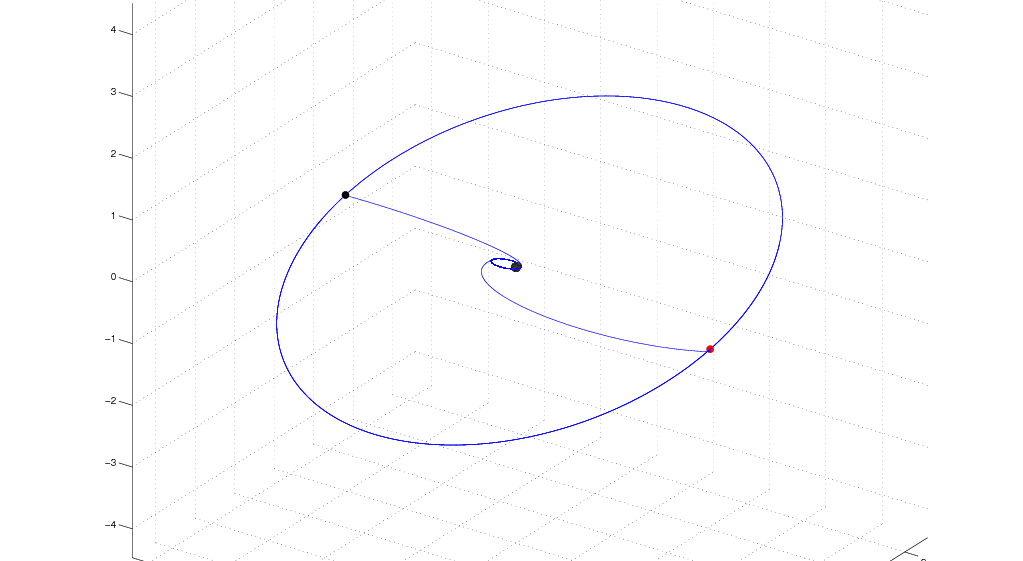
\includegraphics[width=\textwidth]{orbits.png}
  \caption{The outer ring is the lunar orbit and the inner ring is a
simplified version of the satellite's orbit which does not account for
the influence of the moon's gravity. The two otter dots represent
potential impact points (red is the ascending first node and black is
the descending second node) and the lines coming away from the earth
represent the possible trajectories of the satellite to the impact points.}
  \label{fig:orbitssimp}
\end{figure}

After some guess work with the $\Delta v$ values from both launch
points, they were found to be 0.703 km/s from perigee and 2.544 km/s
from apogee. The perigee launch would get the satellite within 759. m
of the second impact point in $2.197 \times 10^5$ s. And the other
launch would put the satellite 678. m from the first impact point in
$4.126 \times 10^5$ s.

From this it is clear that launching from perigee makes most sense
both time wise and financially since less fuel would be needed.
Now, in order to implement the improved equations of motion
(Equation.(\ref{eq:eom})),
we first have to decide when to launch the satellite. Since the time
it takes for the moon to get to the second impact point is known from
the event that determined the impact point's location, $2.312\times
10^6$ s, the that it takes the satellite to get to the second impact
point from perigee can be subtracted from that time to determine when
the satellite should be launched. That is, $2.0924\times 10^6$ s from
when the moon is at perigee. Knowing this, we can find the
initial conditions for the moon then and plug this into
Equation.(\ref{eq:eom}) to have an accurate picture of what the
trajectory will look like:

\begin{figure}[H]\centering
  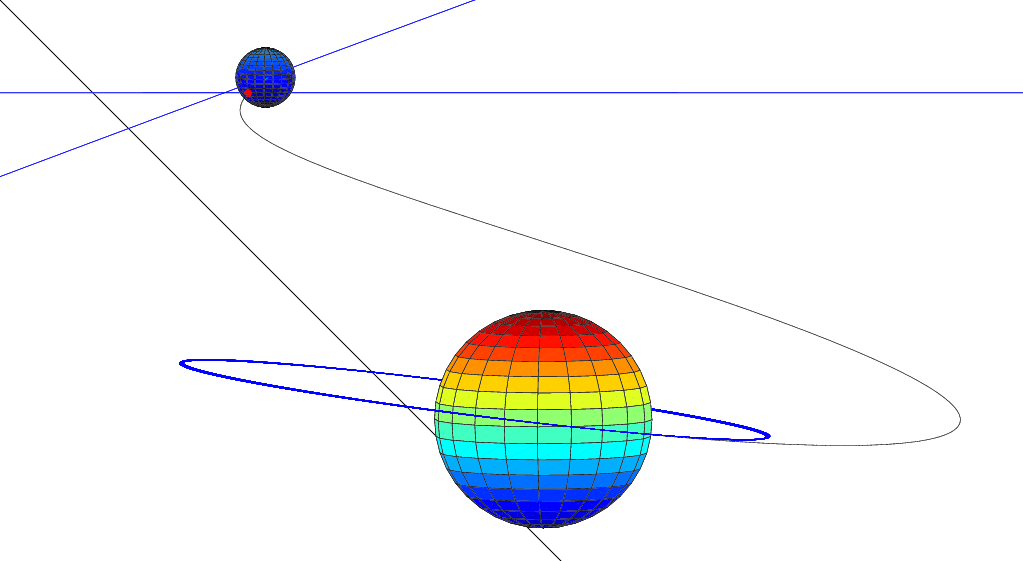
\includegraphics[width=\textwidth]{impact2.png}
  \caption{The black line is the trajectory of the satellite after it
    leaves perigee and makes its journey to the moon (blue orb).}
  \label{fig:impact}
\end{figure}

\section{Conclusions}

The satellite should be launched from perigee at 12:13 am EDT on
Wednesday, April 13, 2011. This will cause a hit at 2:43 am EDT on
Wednesday, April 13, 2011. The velocity change in the satellite should
be 0.703 km/s. The impact velocity will be 2.682 km/s.

\pagebreak
\section{Bibliography}
\begin{thebibliography}{99}
  \bibitem[ENG]{ENG} Engineering Department, Brown University,
    \textsl{Orbital Design for a Lunar Impact Mission: Detailed
Design}, 2011, \\
    {\small
      \texttt{www.engin.brown.edu/courses/en4/Projects/Projects.htm}}
  \bibitem[USNO]{USNO}US Navy,
    \textsl{Naval Oceanography Portal,}\\
    {\small
      \texttt{www.usno.navy.mil/USNO/astronomical-applications/data-services/geo-
        pos}}
\end{thebibliography}


\pagebreak

\appendix
\section{Equations}\label{sec:eomcode}
The simple equation of motion (Equation.(\ref{eq:eomsimp})) described
in Section.\ref{sec:motion}, when put into MatLab looks like:
\begin{verbatim}
% Equation of motion as a functoin of time and a position vector
% and velocity vector
function dwdt = eom(t,w)
  x=w(1); y=w(2); z=w(3);
  vx=w(4); vy=w(5); vz=w(6);
  r = sqrt(x^2+y^2+z^2);
  dwdt = [vx;vy;vz;-mu*x/r^3;-mu*y/r^3;-mu*z/r^3];
end
\end{verbatim}

\noindent
The second equation of motion, with the 12 variables looks like:
\begin{verbatim}
% The new and improved equation of motion that solves for the                                                                              
% effect of the moon's gravity on the satellite                                                                                            
function dWdt = eom2(t,w)                                                                                                                  
  xs=w(1); ys=w(2); zs=w(3);                                                                                                               
  vxs=w(4); vys=w(5); vzs=w(6);                                                                                                            
  xm=w(7); ym=w(8); zm=w(9);                                                                                                               
  vxm=w(10); vym=w(11); vzm=w(12);                                                                                                         
  rs = sqrt(xs^2+ys^2+zs^2);                                                                                                               
  rm = sqrt(xm^2+ym^2+zm^2);                                                                                                               
  rmosat = sqrt((xm-xs)^2+(ym-ys)^2+(zm-zs)^2);                                                                                            
  % kappa is the ratio between the moon's mass and the earth's                                                                             
  dWdt = [vxs;vys;vzs;...                                                                                                                  
          -mu*xs/rs^3+mu*kappa*(xm-xs)/rmosat^3;...                                                                                        
          -mu*ys/rs^3+mu*kappa*(ym-ys)/rmosat^3;...                                                                                        
          -mu*zs/rs^3+mu*kappa*(zm-zs)/rmosat^3;...                                                                                        
          vxm;vym;vzm;...                                                                                                                  
          -mu*xm/rm^3;-mu*ym/rm^3;-mu*zm/rm^3];                                                                                            
end
\end{verbatim}

\section{Data Processing}
\subsection{Lunar Orbit}\label{sec:moonorb}
The script, \verb[moondata[, that handled the data taken from the USNO website to find
the initial conditions for the equations of motion is:
\begin{verbatim}
function [rp,vp,perigee,apogee] = moondata(file,grav_par,moonrad)

% Converts degrees to radians
radians = @ (degrees) degrees*pi/180;

% Reads a csv and makes it an array
moondata = csvread(file);

% Stores the perigee and apogee and where they happen
[perigee,pind] = min(moondata(:,8));
[apogee,aind] = max(moondata(:,8));

perigee = perigee + moonrad;
apogee = apogee + moonrad;

% Stores the ra and dec at perigee and apogee
[ra_p,dec_p] = radec(pind);
[ra_a,dec_a] = radec(aind);

% Makes the position vectors at perigee and apogee.
rp = rvec(ra_p,dec_p,perigee);
ra = rvec(ra_a,dec_a,apogee);

% Crosses the position vectors at perigee and apogee to find a
% vector normal to the moon's plane
m = cross(rp,ra)./(norm(cross(rp,ra)));

% Finds velocity when moon is at perigee
vp = sqrt(2*grav_par*apogee/(perigee*(apogee+perigee))) * ...
     (cross(m,rp)/perigee);

% Function that outputs a position vector given the distance, ra,
% and dec (in radians)
function r = rvec(ra,dec,dist)
  r = dist * ...
      [cos(ra)*cos(dec), sin(ra)*cos(dec), sin(dec)];
end


% Function that outputs the ra and dec in radians for a given index
% of moondata.csv
function [ra,dec] = radec(index)
  % Stores the ra and dec in the file as some variables
  ra_deg = moondata(index,1:3);
  dec_deg = moondata(index,4:7)*moondata(index,4);  

  % Converts ra_deg first to decimal degrees
  ra = ra_deg(1)*(360/24) + ...
       ra_deg(2)*360/(24*60) + ...
       ra_deg(3)*60/(24*60*60);
  % Then to radians and stores it as the output of the function
  ra = radians(ra);
  
  % Converts dec values in the file to decimal degrees then radians
  % and stores it as the second output of the function
  dec = dec_deg(2) + dec_deg(3)/60 + dec_deg(4)/(60*60);
  dec = radians(dec);
end

end
\end{verbatim}

\subsection{Satellite Orbit}\label{sec:satorb}
To process the information about Ariane V into initial conditions for
the satellite:
\begin{verbatim}
function [rp,vp,normalvector] = satellite(inc,peri_alt,apo_alt,arg,long,rb,grav_par)

radians = @ (degrees) degrees*pi/180;

inc = radians(inc);
arg = radians(arg);
long = radians(long);

peri_alt = peri_alt + rb;
apo_alt = apo_alt + rb;

rp = (peri_alt) * ...
     [ (cos(arg)*cos(long)-sin(arg)*sin(long)*cos(inc)), ...
       (cos(arg)*sin(long)+sin(arg)*cos(long)*cos(inc)), ...
       (sin(arg)*sin(inc)) ];

vp = sqrt(2*grav_par*apo_alt/(peri_alt*(apo_alt+peri_alt))) * ...
     [ -(sin(arg)*cos(long)+cos(arg)*sin(long)*cos(inc)), ...
     (cos(arg)*cos(long)*cos(inc)-sin(arg)*sin(long)), ...
     (cos(arg)*sin(inc)) ];

normalvector = [sin(long)*sin(inc), -cos(long)*sin(inc), cos(inc)];

end
\end{verbatim}

\section{Implementations}\label{sec:events}

A series of MatLab event functions were used to extract various
necessary pieces of information:
\begin{verbatim}
function [event_val,stopthecalc,direction] = ...
    detect_impact_point1(t,w)
  % Position vector of moon (this assumes w(1)=x,w(2)=y,w(3)=z)
  r = w(1:3);
  % Detect when r.n=0
  event_val = dot(n,r);
  stopthecalc = 0;
  direction = 0;
end

% Finds the initial conditions for when the satellite is at apogee to
% determine it's trajectory to the first impact point.
function [event_val,stopthecalc,direction] = satapogee(t,w);
  event_val = sqrt(w(1)^2+w(2)^2+w(3)^2)-(apo_sat+re);
  stopthecalc = 0;
  direction = 0;
end

function [tvals,wvals,test_d,time_to_reach] = minimum(t,w,r_imp)
  options = odeset('RelTol',0.00000001,'Event',@min_dist);
  [tvals,wvals,tevent,wevent] = ...
      ode45(@eom,[0,t],w,options);
 
  [test_d,time_to_reach] = ...
      mindisttomoon(tevent,wevent,r_imp);

  function [event_val,stopthecalc,direction] = ...
      min_dist(t,w)
    event_val = dot((r_imp - transpose(w(1:3))),w(4:6));
    stopthecalc = 1;
    direction = 0;
  end

  function [d,time_to_reach_min] = ...
      mindisttomoon(t_event,w_event,r_impact)
    rmin = w_event(1,1:3)-r_impact;
    d = sqrt(dot(rmin,rmin)); % min dist to moon.
    time_to_reach_min = tevent(1); % Time to reach the min dist.
  end

% This funciton determines when the satellite hits the surface of the moon
function [event_val,stopthecalc,direction] = stopper(t,w)
  r = sqrt((w(7)-w(1))^2+(w(8)-w(2))^2+(w(9)-w(3))^2);
  event_val = r - moon_radius;
  stopthecalc = 1;
  direction = 0;
end
\end{verbatim}

\end{document}
